%!TEX program = xelatex
\documentclass[UTF8]{beamer}
\usepackage{mathtools}
\usepackage{graphicx}
\usepackage{amsmath}
\usepackage{xeCJK}
\setCJKmainfont{SimSun}
\setCJKsansfont{黑体}
\usetheme{Madrid}

\newcommand\myeq{\stackrel{\mathclap{\tiny\mbox{def}}}{=}}
\DeclareMathOperator*{\argmin}{arg\,min}
% \usepackage{beamerthemesplit} // Activate for custom appearance

\title{Understanding Black-box Predictions via Influence Functions}
\author{Pang Wei Koh \& Percy Liang}

\date{\today}

\begin{document}

\frame{\titlepage}

\section[Outline]{}
\frame{\tableofcontents}

\section{Introduction}
\begin{frame}
\frametitle{The problem}
\begin{itemize}
\item Classification problem: $\mathcal{X} \mapsto \mathcal{Y}$, where $\mathcal{X}\in\mathbb{R}^M$ and $\mathcal{Y}\in\{+1, -1\}$.\\
\item Training instances $z_1,\dots, z_n$, where $z_i = (x_i, y_i) \in \mathcal{X}\times\mathcal{Y}$\\
\item Empirical loss is $L(z, \theta) = \frac{1}{n}\sum_{i=1}^{n}L(z_i, \theta)$, 
\item $\hat{\theta} \myeq \argmin_{\theta\in\Theta}\frac{1}{n}\sum_{i=1}^nL(z_i, \theta)$
\end{itemize}
Assume $L(z, \theta)$ is twice-differentiable and strictly convex in $\theta$.

If we remove $z$ from the training data, the change on parameter is $\Delta = \hat{\theta}_{-z} - \hat{\theta}$, where:
\begin{align}
% \hat{\theta} &\myeq \argmin_{\theta\in\Theta}\frac{1}{n}\sum_{i=1}^nL(z_i, \theta) \nonumber\\
\hat{\theta}_{-z} &\myeq \argmin_{\theta\in\Theta}\sum_{z_i\neq z}L(z_i, \theta) \nonumber
\end{align}
Retraining the model in leave-one-out scheme is prohibitively slow.
\end{frame}

\section{Approach}
\begin{frame}
\frametitle{Influence on the parameters $\theta$}
Let $\hat{\theta}_{\epsilon, z}$ the parameters if $z$ were up-weighted by some small $\epsilon$:
\begin{equation} \nonumber
\hat{\theta}_{\epsilon, z} \myeq \argmin_{\theta\in\Theta}\frac{1}{n}\sum_{i=1}^nL(z_i, \theta) + \epsilon L(z, \theta)
\end{equation}

The influence of up-weighting $z$ on the parameters $\hat\theta$ is
\begin{equation}
\mathcal{I}_{up,params}(z)\myeq\frac{d\hat{\theta}_{\epsilon, z}}{d\epsilon}\vert_{\epsilon=0} = -H^{-1}_{\hat{\theta}}\nabla_\theta{}L(z, \hat{\theta}) 
\end{equation}
where, $H_{\hat\theta} \myeq \frac{1}{n}\sum_{i=1}^n\nabla^2_{\theta}L(z_i, \hat\theta)$

Removing $z$ is the same as $\epsilon = -\frac{1}{n}$, then (by linear approximation)
\begin{equation}
\Delta = \hat{\theta}_{-z} - \hat{\theta} \approx -\frac{1}{n}\mathcal{I}_{up,params}(z) \nonumber
\end{equation}
\end{frame}

\begin{frame}
\frametitle{Influence on the test loss $L(z_{test}, \theta)$}
What is the influence on the loss at a test point $z_{test}$ by upweighting $z$ ?
\begin{align}
\mathcal{I}_{up,loss}(z, z_{test}) & \myeq\frac{dL(z_{test}, \hat\theta_{\epsilon, z})}{d\epsilon}\vert_{\epsilon=0}  \nonumber\\ 
& = \nabla_{\theta}L(z_{test}, \hat{\theta})^T\times \frac{d\hat\theta_{\epsilon, z}}{d\epsilon}\vert_{\epsilon=0}  \nonumber \quad \textnormal{\small(apply the chain rule)} \\
& = \nabla_\theta{}L(z_{test}, \hat\theta)^T\times (-H_{\hat\theta}^{-1}\nabla_{\theta}L(z, \hat\theta))\nonumber \\
& = \nabla_\theta{}L(z_{test}, \hat\theta)^T\times \mathcal{I}_{up,params}(z) \nonumber
\end{align}

Influence on $z_{test}$ by upweigting $z$:
\begin{equation}
\mathcal{I}_{up,loss}(z, z_{test}) = -\nabla_\theta{}L(z_{test}, \hat\theta)^TH_{\hat\theta}^{-1}\nabla_{\theta}L(z, \hat\theta)
\end{equation}
\end{frame}
\begin{frame}
\frametitle{Perturbing a training instance}
A train instance $z = (x, y)$, define a new instance $z_\delta \myeq (x + \delta, y)$. 
\begin{center}
If $z \mapsto z_\delta$, what is the change on $\theta$?
\end{center}

By definition,
\begin{equation}\nonumber
\hat\theta_{\epsilon, z_{\delta}, -z} \myeq \argmin_{\theta\in\Theta} \frac{1}{n}\sum_{i=1}^{n}L(z_i, \theta)+\epsilon L(z_\delta, \theta) - \epsilon L(z, \theta)
\end{equation}
And we obtains
\begin{align}
\frac{d\hat\theta_{\epsilon, z_\delta, -z}}{d\epsilon}\vert_{\epsilon = 0} &= \mathcal{I}_{up, params}(z_\delta) - \mathcal{I}_{up, params}(z) \nonumber\\
&= -H_{\hat\theta}^{-1}(\nabla_{\theta}L(z_\delta, \hat\theta) - \nabla_{\theta}L(z, \hat\theta))
\end{align}
%\begin{equation}
%\Delta = \hat\theta_{z_\delta, -z} - \hat\theta \approx \frac{1}{n}(\mathcal{I}_{up,params}(z_\delta) - \mathcal{I}_{up, params}(z))
%\end{equation}
\end{frame}
\begin{frame}
\frametitle{Perturbing influence on the test loss}
What is the influence on the loss at a test point $z_{test}$ by perturbing $z$ ?
\begin{align}
\mathcal{I}_{pert, loss}(z, z_{test})^\top &\myeq \nabla_{\delta}L(z_{test}, \hat\theta_{z_\delta, -z})^\top\vert_{\delta=0} \nonumber\\
&= -\nabla_{\theta}L(z_{test}, \hat\theta)^TH_{\hat\theta}^{-1}\nabla_x\nabla_{\theta}L(z, \hat\theta)
\end{align}
$\mathcal{I}_{pert, loss}(z, z_{test})^\top\delta$ tells us the approximate effect that $z\mapsto z+\delta$ has on the loss at $z_{test}$.\\
By setting $\delta$ in the direction of $\mathcal{I}_{pert, loss}(z, z_{test})$, we can construct local perturbations of $z$ that maximally increase the loss at $z_{test}$.
\end{frame}
\begin{frame}
\frametitle{Brief Summary}
$\mathcal{I}_{up,params}(z)$描述的是对一个训练样本$z$,增加$\epsilon$的权重后,对模型参数的影响
\begin{equation}
\mathcal{I}_{up,params}(z)\myeq\frac{d\hat{\theta}_{\epsilon, z}}{d\epsilon}\vert_{\epsilon=0} = -H^{-1}_{\hat{\theta}}\nabla_\theta{}L(z, \hat{\theta}) \nonumber
\end{equation}
$\mathcal{I}_{up,loss}(z, z_{test})$描述的是对$z$增加$\epsilon$权重后,对模型在测试样本$z_{test}$上的loss的影响
\begin{equation}
\mathcal{I}_{up,loss}(z, z_{test}) = -\nabla_\theta{}L(z_{test}, \hat\theta)^TH_{\hat\theta}^{-1}\nabla_{\theta}L(z, \hat\theta) \nonumber
\end{equation}
$\mathcal{I}_{pert, loss}(z, z_{test})$描述的是对训练样本$z$本身做修改$\delta$,对模型在测试样本$z_{test}$上的loss的影响
\begin{equation}
\mathcal{I}_{pert, loss}(z, z_{test})^\top = -\nabla_{\theta}L(z_{test}, \hat\theta)^TH_{\hat\theta}^{-1}\nabla_x\nabla_{\theta}L(z, \hat\theta) \nonumber
\end{equation}
\end{frame}
\section{Efficiently Calculating Influence(略过)}
\section{Validation experiments}
\begin{frame}
\frametitle{Influence functions vs. leave-one-out retraining}
\begin{center}
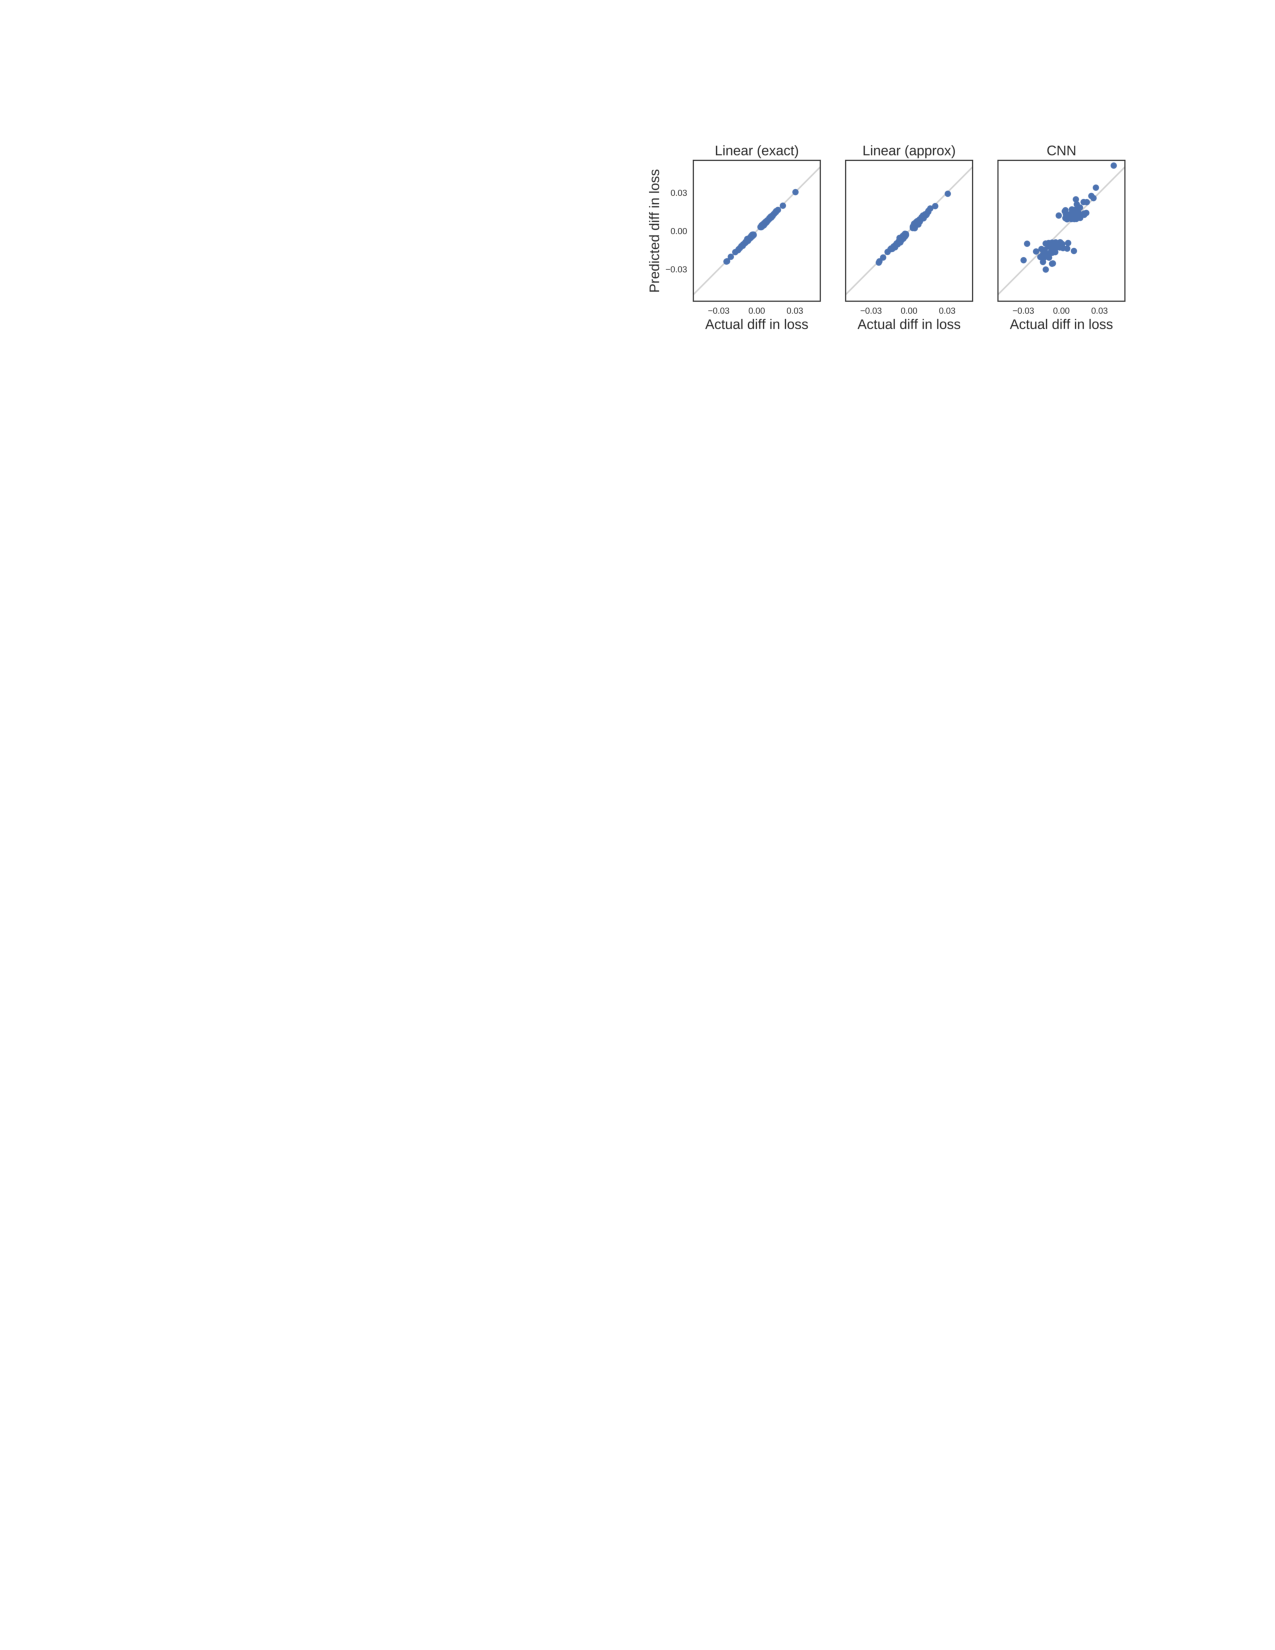
\includegraphics[width=0.5\textwidth]{corr.pdf}
\end{center}
\begin{itemize}
\item 图1:精确计算inverse HVP vs. leave-one-out retraining LR
\item 图2:近似计算inverse HVP vs. leave-one-out retraining LR
\item 图3:即使在CNN (non-convergent, non-convex)的情况下,IF的计算结果仍然有意义。(Pearson's R=0.86)
\end{itemize}
\end{frame}

\begin{frame}
\frametitle{Retraining with less harmful instance}
这里使用jxjAModel-v1.1模型的上线版本,使用test集合整体来计算训练样本的influence,将有害样本依次剔除,重新训练模型并且评估效果。
\begin{center}
\begin{tabular}{ | c | c | c | }
  \hline
  Train with & Gini on test & Gini on OOT \\ \hline            
  All & 55.31 & 53.32 \\ \hline      
  -1 & 55.43 & 53.36 \\ \hline      
  -10 & 55.66 & 53.46 \\ \hline
  - 500 & 60.00 & 53.31 \\ \hline
  - 1000 & 61.14 & 51.97 \\ \hline
  - 5000 & 61.90 & 49.15 \\ \hline
  - 1w & 61.36 & 46.47 \\ \hline
\end{tabular}
\end{center}
测试集合效果提升很快,说明influence的计算结果是有意义的;\\
OOT上的效果略升后下降,说明通过这种方式剔除样本会使训练集合向测试集合样本分布拟合,从而降低了模型泛化能力。
\end{frame}

\section{Use cases}
\begin{frame}
\frametitle{Understanding model behavior(模型行为的可解释性)}
选取一个测试图片(图左上角),分别计算SVM和NN模型训练样本的influences,并挑选最重要的两个样本。
\begin{columns}[T]
\begin{column}{.48\textwidth}
作者通过这个实验来说明SVM模型与NN模型prediction的依据不同。
\begin{itemize}
\item SVM模型看上去主要依据像素距离(颜色分布)
\item NN模型可能更依据图像的纹路特征
\end{itemize}
\end{column}
\hfill%
\begin{column}{.48\textwidth}
\begin{tabular}{c}
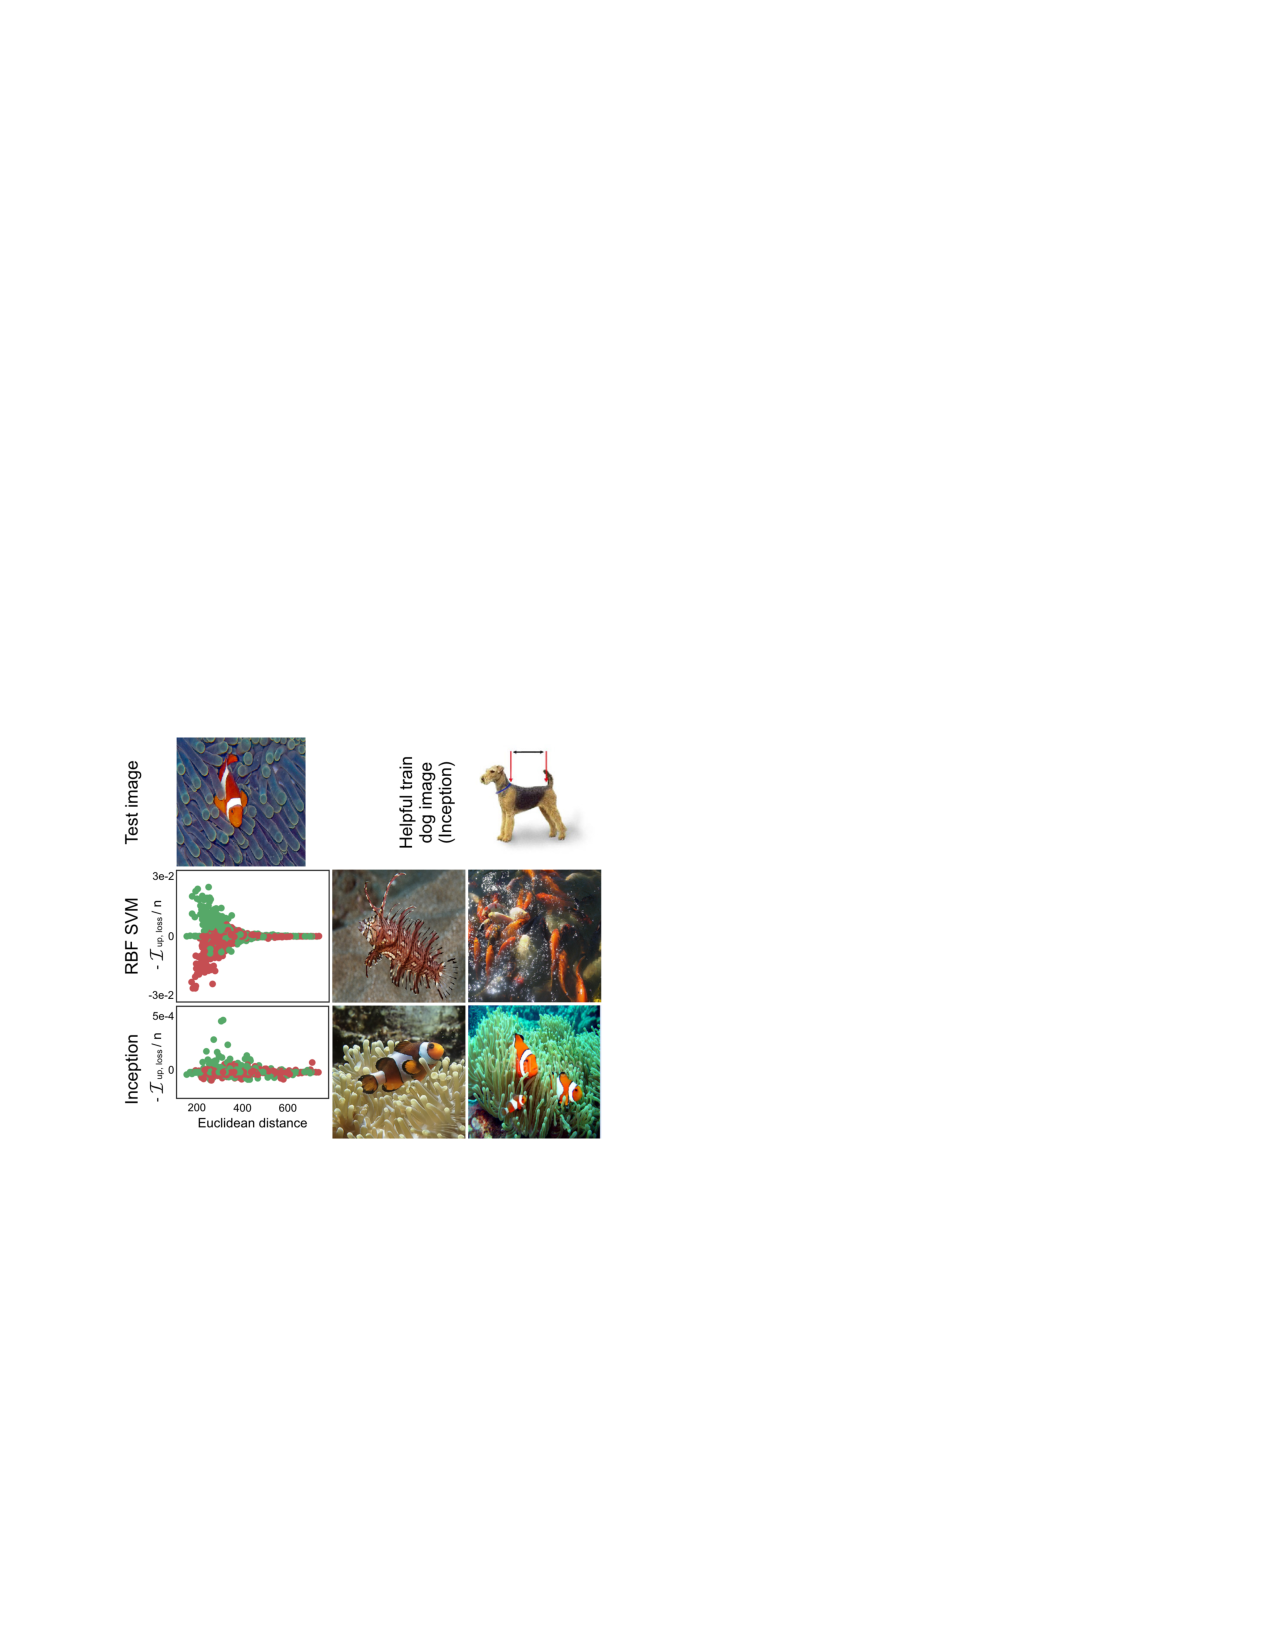
\includegraphics[width=0.8\textwidth]{fish.pdf}
\end{tabular} 
\end{column}%
\end{columns}
同时,作者也给出了反例,(如图右上角),狗由于身上的纹路与测试样本相似,因此也对预测有帮助(wtf?)
\end{frame}
\begin{frame}
\frametitle{Training attacks(机器学习模型的安全性)}
\begin{center}
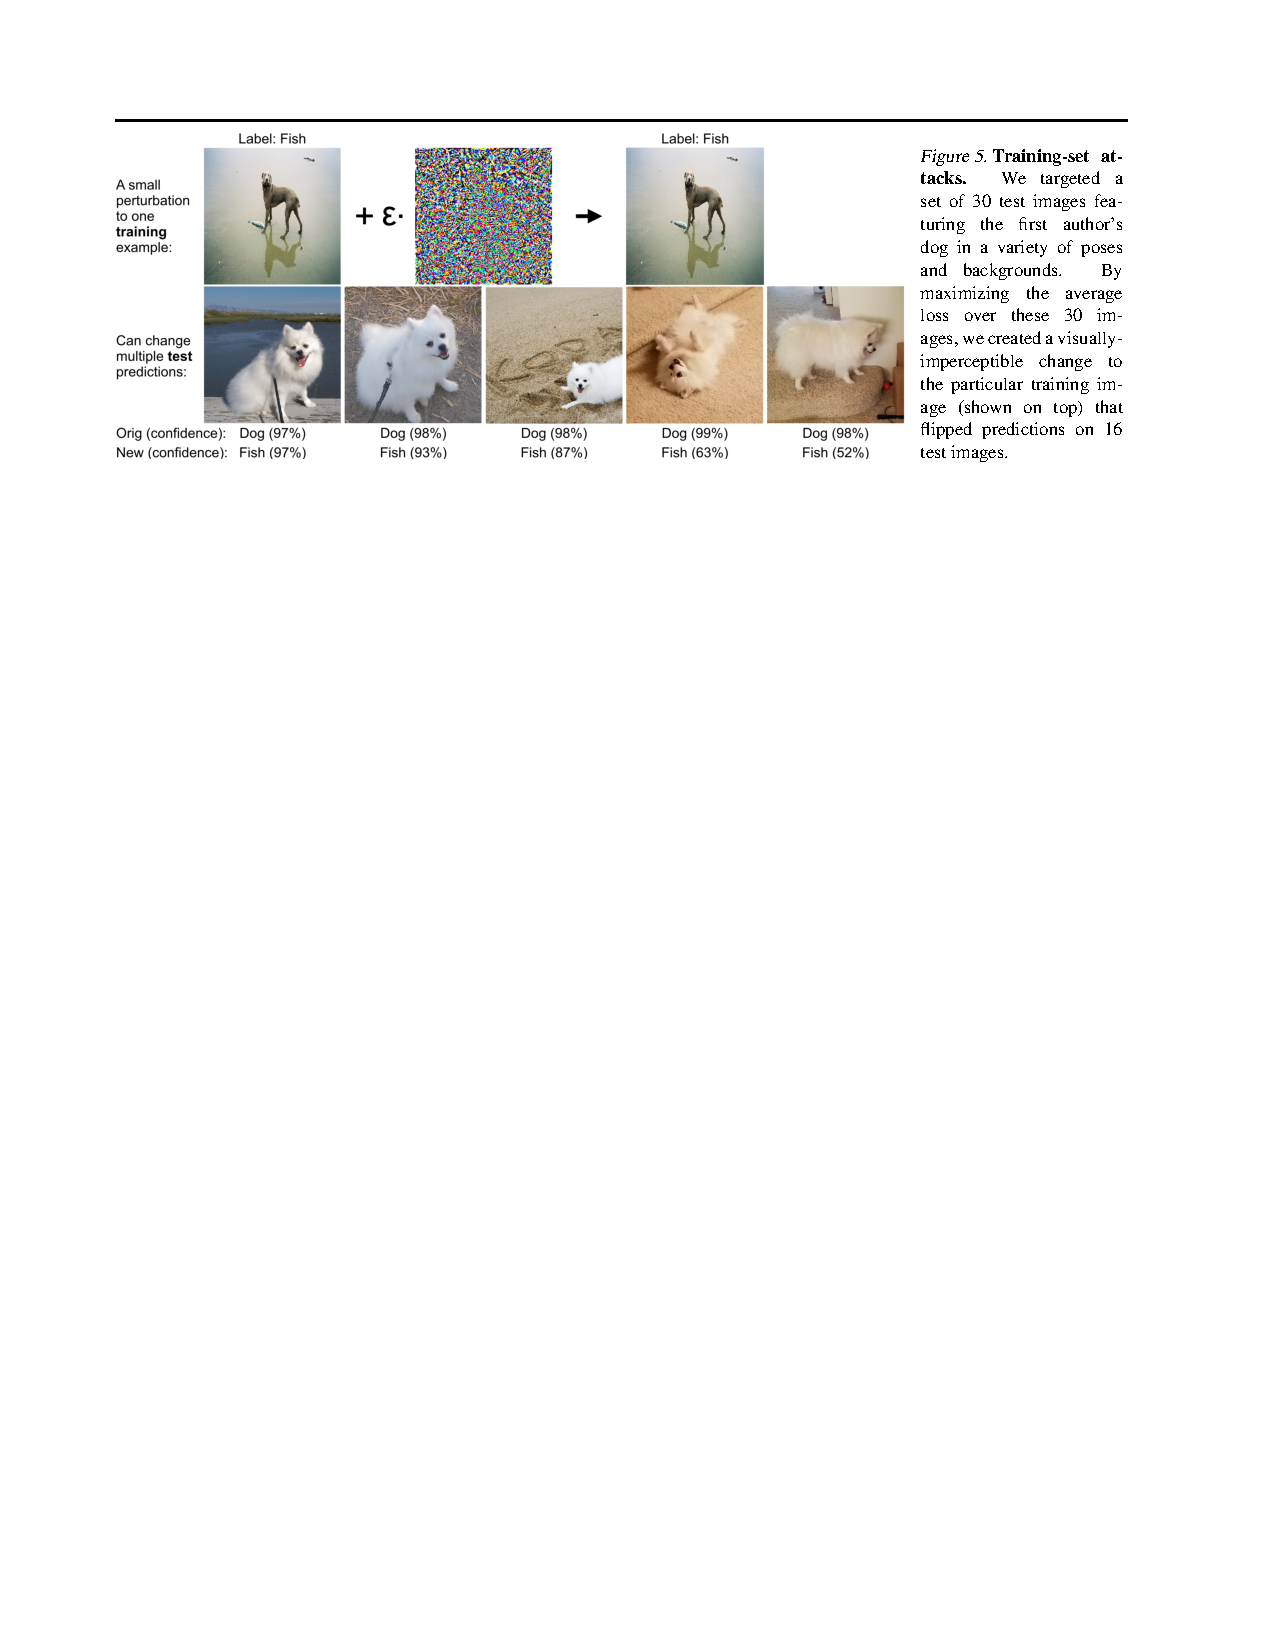
\includegraphics[width=0.9\textwidth]{cat.pdf}
\end{center}
这个实验描述的是,如果在关键样本上增加一点肉眼无法察觉的噪音扰动,可以对模型的预测结果产生很大的影响。
\end{frame}

\begin{frame}
\frametitle{Debugging domain mismatch(分布不一致问题)}
度学金语言模型;任意挑选一个“坏人”Fico分高的样本;通过InfluenceFunction找出影响模型打分最重要的“有害"训练样本;进而找出哪些特征造成了该Influence。
\begin{center}
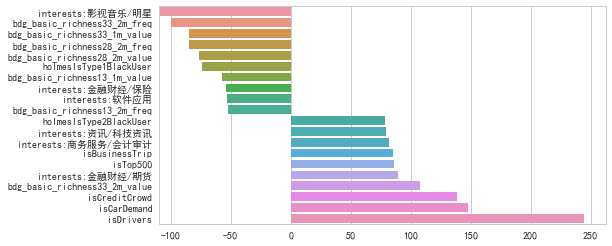
\includegraphics[width=0.8\textwidth]{gradInf.png}
\end{center}
\begin{center}
\tiny
\begin{tabular}{ | c | c | c | c | c | c | c |}
\hline
Feature & \multicolumn{2}{c|}{isDrivers} & \multicolumn{2}{c|}{isCarDemand} & \multicolumn{2}{c|}{isCreditCrowd} \\
{} & Trn & oot & Trn & oot &  Trn & oot \\ \hline
woe:0 & 0.0011 & {\color{red}0.0202} & 0.0009 & {\color{red}0.0148} & 0.0018 & {\color{red}0.038} \\ \hline
woe:1 & -1.1219 & -0.4208 & -0.4442 & -0.2089 & -0.6318 & -0.5618 \\ \hline 
iv & 0.0012 & 0.0084 & 0.0004 & 0.0031 & 0.0011 & 0.0213 \\ \hline
\end{tabular}
\end{center}
\end{frame}

\begin{frame}
\frametitle{Fixing mislabeled examples(样本标签问题)}
作者在垃圾邮件分类模型中,随机挑选10\%的样本改变标签,用来模拟实际数据中的样本噪音。并且希望通过Influence来定位可疑样本,并通过人工review的方式来修正样本,改善模型。
\begin{columns}[T]
\begin{column}{.48\textwidth}
三种方式对比:
\begin{itemize}
\item 随机抽取数据来review(红色):费时低效
\item 选取train loss较高的样本来review(绿色)
\item 选取influence有害的样本来review(蓝色)
\end{itemize}
\end{column}
\hfill%
\begin{column}{.48\textwidth}
\begin{tabular}{c}
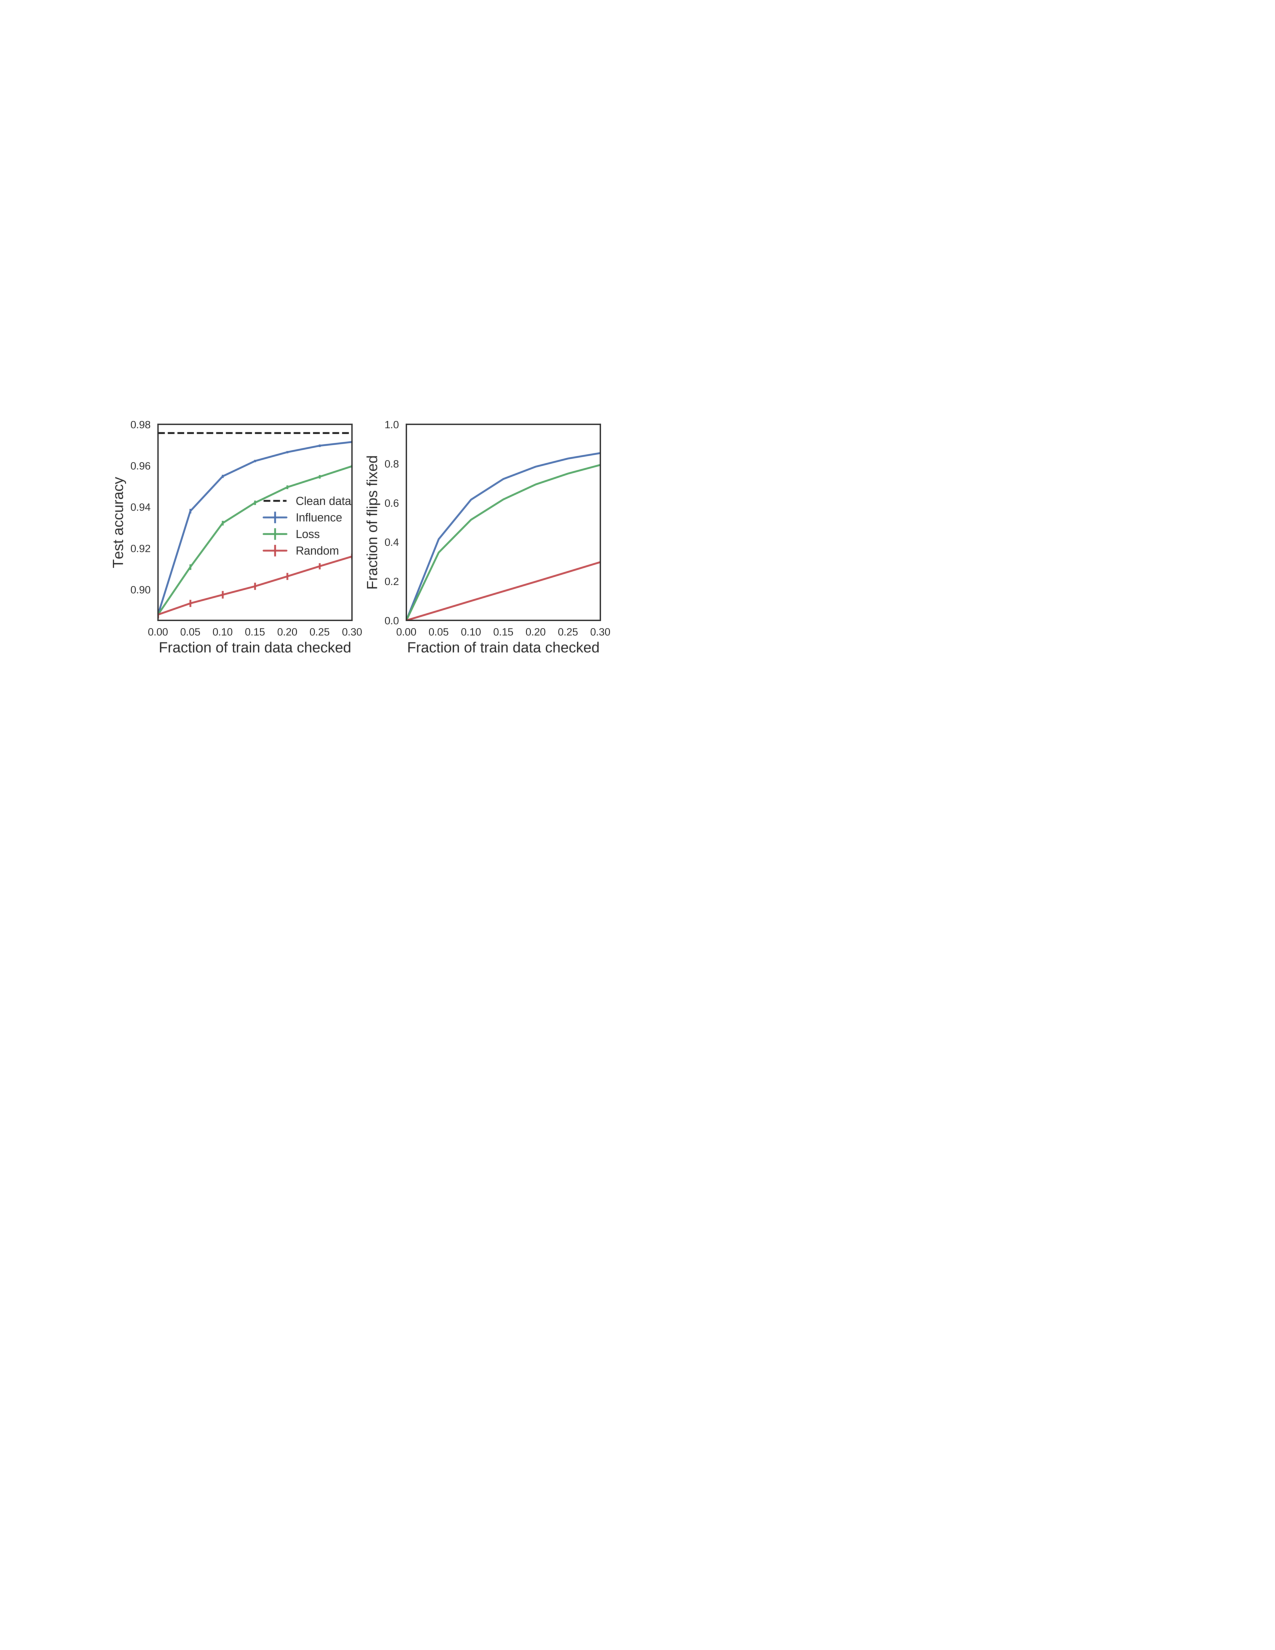
\includegraphics[width=0.95\textwidth]{flip.pdf}
\end{tabular} 
\end{column}%
\end{columns}
\end{frame}
\end{document}
